\documentclass[a4paper,11pt]{article}
\usepackage[osf]{mathpazo}
\usepackage{ms}
\usepackage[]{natbib}
\raggedright

\newcommand{\smurl}[1]{{\footnotesize\url{#1}}}
\usepackage{graphicx}

\title{What we don't currently know about global plant functional diversity}
\author{
Will Cornwell$^1$
et al.}

\affiliation{
*final list and order undecided\\
$^1$ University of NSW\\
}
\date{}

\bibliographystyle{mee}

\usepackage[title,titletoc,toc]{appendix}

\mstype{Research Article}
\runninghead{What we don't know}
\keywords{}

\begin{document}
\mstitlepage
\noindent
% \doublespacing
% \linenumbers

\section{Summary}


\section{Introduction}




\section{Methods}


\section{Results}

\section{Discussion}

Data interpolation techniques rely principally on phylogenetic relatedness.  
Most, models of the expected similarity based on relatedness rely on an underlying implicit or explicit model of trait evolution.  
Usefully some of the recently proposed methods do allow for characterising uncertainty, this uncertainty in the typical case
does not include model uncertainty.  And as most simple models of trait evolution for plants are far from adequate (Pennell), 
we have a ways to go before we fully understand uncertainty in trait imputation approaches.   


\section{Figures}

\begin{figure}[h!]
\centering
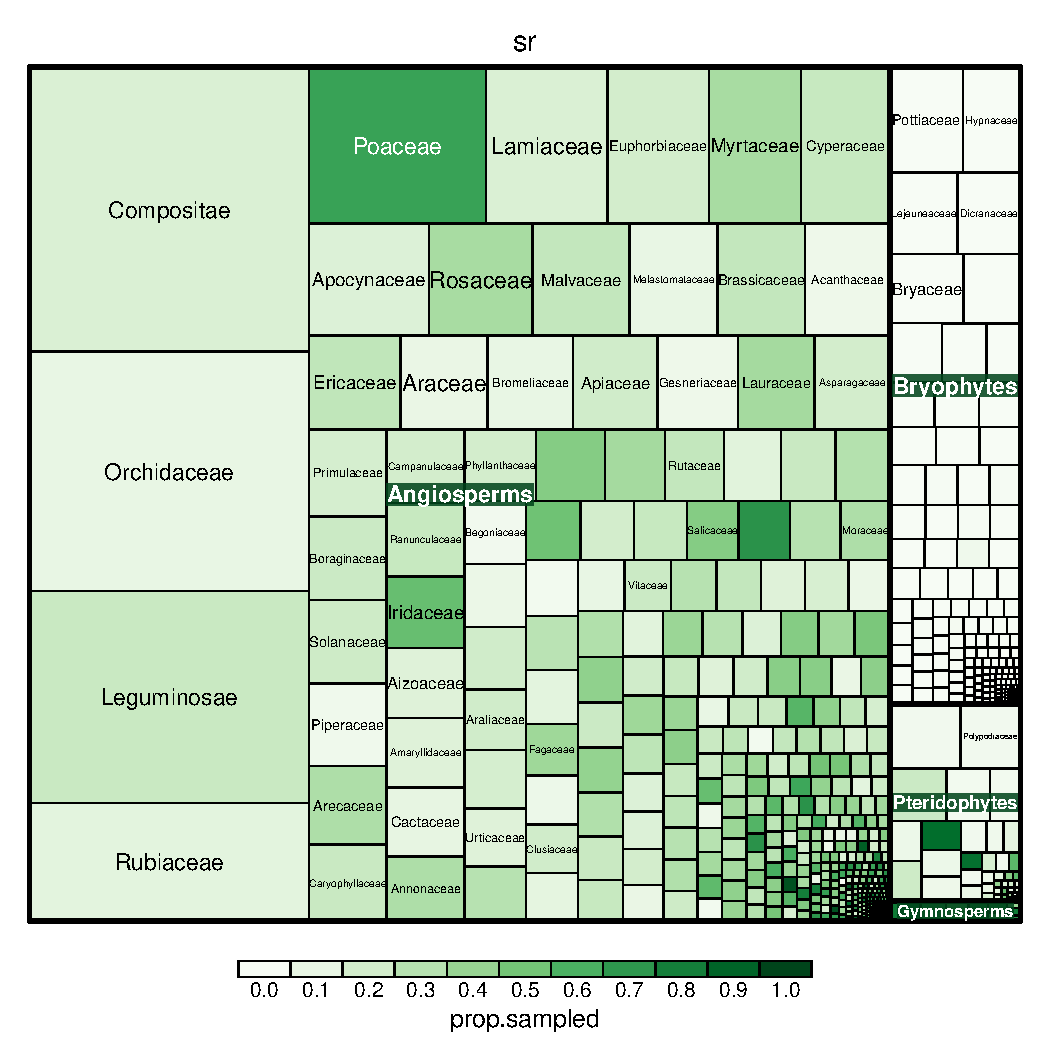
\includegraphics[width=15cm,height=15cm,keepaspectratio]{figures/sampling_in_try_by_family.pdf}
\caption{Algorithm for modelling dynamics within the ``mature'' male population.}
\label{fig:events}
\end{figure}
\clearpage

\bibliography{refs}

\end{document}

